\section{Derivations}


\subsection{Mean and covariance of integral of Brownian motion}
\label{app:intBM}
Shifted Brownian motion is defined as a Gaussian process $\nu(t)$ on $t \geq 0$, with mean and covariance functions defined as
\be
	m^{(\nu)}(t) = \nu_0
	\quad,\qquad 
	K^{(\nu)}(t, t') = D\,\text{min}(t, t')\quad,
\ee
where $\nu_0$ is the starting point at $t = 0$, and $D$ is the diffusion coefficient of the Brownian motion.

We define the integral of the Brownian motion as the process $\mu(t) = \mu_0 + \intop_0^t \d{x} \nu(x)$ on $t \geq 0$, with mean and covariance functions defined as
\be
	m^{(\mu)}(t) = \mu_0 + \intop_0^{t} \d{x} m^{(\nu)}(x) = \mu_0 + \nu_0 t
	\quad,\qquad
	K^{(\mu)}(t, t') = \intop_0^t \d{x} \intop_0^{t'} \d{y} K^{(\nu)}(x, y)
\ee
Since $K^{(\nu)}(x,y) = D\,\text{min}(x,y)$ is symmetric in its arguments, with the notation $l = \text{min}(t, t')$ and $h = \text{max}(t, t')$, we can write 
\be
	K^{(\mu)}(t, t') = D\intop_0^h \d{x} \intop_0^{l} \d{y} \text{min}(x, y)
\ee
 The integration domain can be partitioned into three non-overlapping domains,
\begin{figure}[h]
\centering
	\includegraphics[width=0.3\textwidth]{figs/I1I2I3_regions.pdf}
\end{figure}
\ba
	I_1 &=& \intop_0^l \d{x} \intop_0^x \d{y} \underbrace{\text{min}(x,y)}_{y} \;=\; \intop_0^l \d{x} \frac{x^2}{2} \;=\; \frac{l^3}{6}
	\\
	I_2 &=& \intop_0^l \d{y} \intop_0^y \d{x} \underbrace{\text{min}(x,y)}_{x} \;=\; \intop_0^l \d{y} \frac{y^2}{2} \;=\; \frac{l^3}{6}
	\\
	I_3 &=& \intop_l^h \d{x} \intop_0^l \d{y} \underbrace{\text{min}(x,y)}_{y} \;=\; \intop_l^h \d{x} \frac{l^2}{2} \;=\; (h-l)\frac{l^2}{2}
\ea
the sum of which yields
\be
	K^{(\mu)}(t, t') = D(I_1 + I_2 + I_3) = D\,\frac{l^2}{2}\left(h - \frac{l}{3}\right)  = D\,\frac{\text{min}(t, t')^2}{2}\left(\text{max}(t, t') - \frac{\text{min}(t, t')}{3}\right)
\ee

\subsection{Gaussian integral}
\label{app:gaussian_integral}
Here we calculate the following multi-dimensional Gaussian integral, where $z, \mathcal{B} \in \mathds{R}^n$, $\mathcal{A}\in \mathds{R}^{n\times n}$ (positive definite) and $\mathcal{C} \in \mathds{R}$, 
\ba
	I &:=& \int\d{z} \exp\left(-\frac{1}{2}z\T \mathcal{A} z + \mathcal{B}\T z + \mathcal{C}\right) \\
	&= &
	\int\d{z} \exp\left(-\frac{1}{2}z\T \mathcal{A} z + \frac{1}{2}z\T \mathcal{B} + \frac{1}{2}\mathcal{B}\T z + \mathcal{C}\right) \\
	&=&
	\int\d{z} \exp\left(-\frac{1}{2}\Big(z - \mathcal{A}^{-1}\mathcal{B}\Big)\T \mathcal{A} \Big(z - \mathcal{A}^{-1}\mathcal{B}\Big) + \frac{1}{2}\mathcal{B}\T\mathcal{A}^{-1}\mathcal{B} + \mathcal{C}\right)\\
	&=&
	\exp\left(\frac{1}{2}\mathcal{B}\T\mathcal{A}^{-1}\mathcal{B} + \mathcal{C}\right) \int\d{z'} \exp\left(-\frac{1}{2}(z')\T \mathcal{A} z'\Big)\right).
\ea
Since $\mathcal{A}$ is positive definite there exists an orthogonal matrix $\mathcal{O}$ that diagonalizes it, 
\be
	\mathcal{OAO}\T = \Lambda = \text{diag}(\lambda_1, \lambda_2, \ldots \lambda_n)
\ee
where $\lambda_i$ are the eigenvalues of $\mathcal{A}$. In terms of the transformed coordinates $z'' = \mathcal{O}z'$ we get a separable integral:
\be
	\int\d{z'} \exp\left(-\frac{1}{2}(z')\T \mathcal{A} z'\Big)\right) = \int\d{z''} \exp\left(-\frac{1}{2}(z'')\T \Lambda z''\Big)\right) = \prod_{i=1}^n \int\d{x_i} \exp\left(-\frac{1}{2}x_i \lambda_i x_i\Big)\right)
\ee
Each factor can be simplified using the result for a 1-dimensional Gaussian integral $\int\d{x}\exp(-\frac{1}{2}ax^2) = \sqrt{2\pi / a}$, giving
\be
	\prod_{i=1}^n \sqrt{2\pi / \lambda_i} = \sqrt{\frac{(2\pi)^n}{\prod_i \lambda_i}} = \sqrt{\frac{(2\pi)^n}{\text{det}(\Lambda)}} = \sqrt{\frac{(2\pi)^n}{\text{det}(\mathcal{A})}},
\ee
where $\det{(\Lambda)} = \det{(\mathcal{A})}$, because the transformation matrix $\mathcal{O}$ is orthogonal, i.e. $\det\mathcal{(O)} = 1$. This results in
\be
	I = \exp\left(\frac{1}{2}\mathcal{B}\T\mathcal{A}^{-1}\mathcal{B} + \mathcal{C}\right)\times \sqrt{\frac{(2\pi)^n}{\text{det}(\mathcal{A})}}\quad.
\ee

\section{Implementation}

\subsection{Heuristic method for detecting jump events}
\label{app:heuristic_method}
Given the raw time point and OD series $(\text{tp}, \text{od})$, we wish to eliminate the intermittent OD spikes, and detect the sudden drops of OD.

\begin{enumerate}
	\item To eliminate the OD spikes, we fit a normal + Cauchy mixture model to the distribution of the logarithm of OD values $x_i = \log(\text{od}_i)$ (while disregarding the time points),
	\be
		P(\{x_i\}) = \prod_{i}\Big[w_1 \times \text{Normal}(x_i\;|\;\mu, \sigma) + w_2 \times \text{Cauchy}(x_i\;|\;m, s)\Big],
	\ee
	where $w_1 + w_2 = 1$ are the mixture weights, $\mu$ and $m$ are the centers, and $\sigma$ and $s$ are the widths of the normal and the Cauchy distributions. We initialize the parameters from
	\begin{itemize}
		\item $\mu_0 = m_0 = $ median of the log-OD values,
		\item $\sigma_0 = 2\times$ inter-quartile range of the log-OD values,
		\item $s_0 = 3\sigma_0$, and
		\item $(w_1, w_2)_0 = (0.8, 0.2)$.
	\end{itemize}
	This choice ensures that, after fitting the parameters $\mu, \sigma, m, s, w_1, w_2$, the normal component captures log-OD values from the typical range, and the Cauchy component captures the outliers above and below the typical range.
	After fitting, we compute the center $c$ and width $d$ of the typical region, with the formulas
	\be
		c = \mu,\qquad d = \sqrt{12} \times \sigma,
	\ee
	which is justified by the expectation that, the typical log-OD values are approximately uniformly distributed between the low and high threshold values. Finally, we eliminate all data points where log-OD is outside the $[c - 1.5 \times d, \; c + 1.5 \times d]$ interval. This produces the cleaned data time series $(t, x)$.

	\item To find the start and end indexes $s(r)$, $e(r)$ of each region $r$ of gradual growth, we iteratively attempt to discover additional sub-regions inside already demarked tentative regions with the following steps.
	\begin{enumerate}
		\item The first set of tentative regions is created by partitioning the time series $(t, x)$ along occasional gaps in data collection. We detect such a gap if the time separation of two consecutive data points is 100 times larger than the average consecutive time separation across the entire series.
		\item For each tentative region, we fit a separate linear model $x_i = at_i + b$ (using linear regression).
		\item We subtract a drift term to cancel \emph{some} of the fitted slope $x_{\text{drifting},i} = x_i - (0.7\, a)t_i$. (The factor 0.7 is empirically found to work well, producing very little false jump events, and not missing any obvious jumps.) And, we fit a monotonically decreasing function (using isotonic regression) to $(t, x_\text{drifting})$ in this region.
		\item This can produce several sub regions, defined by the data points for which the monotonic fit is constant. We add each of these sub-regions to the list of tentative regions (which we will investigate in the next iteration), and return to step (b).
		\item If no sub-regions are found, we add the original region to the list of final regions, unless it is too short, i.e. contains less than 10 data points.
	\end{enumerate}
	The start and (inclusive) end coordinates of the final set of regions are sorted into $s$ and $e$ vectors.

\end{enumerate}



\subsection{Stan code for \refeq{eq:L}}
